\documentclass{article}

\title{Numerical Differentiation: Centered Difference Method and Error Considerations}
\author{Jaden Krause}
\date{September 15, 2026}
\usepackage{float}
\usepackage{graphicx}

\renewcommand{\topfraction}{0.9}         % Allow tables to take up 90% of the top of a page
\renewcommand{\bottomfraction}{0.8}      % Allow tables to take up 80% of the bottom of a page
\renewcommand{\textfraction}{0.05}       % Allow text to squeeze into spaces as small as 5% of a page
\renewcommand{\floatpagefraction}{0.95}  % Only give a table its own blank page if it takes up 95%+ of the area

\begin{document}
\maketitle

\section{Introduction}

Numerical differentiation is fundamental to the study of calculus. It begins to take practical significance
when applied to robotics and computation. Computing derivatives using code presents unique challenges that 
must be considered to ensure accuracy. In this paper, I will analyze forward, backward, and centered difference 
methods for numerical differentiation, compare their accuracy, and discuss the errors that are prevalent in 
computational differentiation.

\section{The Problem}

The function I will be dealing with in this discussion is:
$$ f(x) = \sin(x) - \cos(x) $$
evaluated at $ x = 0 $. Using the centered difference formula:
$$ f'(x) = \frac{f(x + h) - f(x - h)}{2h} $$
The step size ($h$) will be from $10^{-1}$ to $10^{-12}$.
To compare the error between the numerical derivative and the true value, I will use:
$$ f'(x) = \cos(x) + \sin(x) $$ 
for the analytical derivative. Table 1 shows the respective values of '$h$', and the corresponding output and 
absolute error for the centered difference method.

\begin{table}
\centering
\begin{tabular}{|l|c|r|}
\hline
\textbf{\textit{h}} & \textbf{Approximation} & \textbf{Absolute Error} \\ \hline
1.0e-01 & 0.998334166468 & 1.665833531719e-03 \\
1.0e-02 & 0.999983333417 & 1.666658333477e-05 \\
1.0e-03 & 0.999999833333 & 1.666666240574e-07 \\
1.0e-04 & 0.999999998333 & 1.667110005599e-09 \\
1.0e-05 & 0.999999999984 & 1.565336749110e-11 \\
1.0e-06 & 0.999999999973 & 2.675548671505e-11 \\
1.0e-07 & 0.999999999474 & 5.263558477964e-10 \\
1.0e-08 & 0.999999999474 & 5.263558477964e-10 \\
1.0e-09 & 1.000000027229 & 2.722921976783e-08 \\
1.0e-10 & 1.000000082740 & 8.274037099909e-08 \\
1.0e-11 & 1.000000082740 & 8.274037099909e-08 \\
1.0e-12 & 1.000033389431 & 3.338943110975e-05 \\ \hline
\end{tabular}
\caption{Centered Difference Formula Results}
\label{tab:centered_difference_formula_results}
\end{table}

\begin{figure}[htbp]
    \centering
    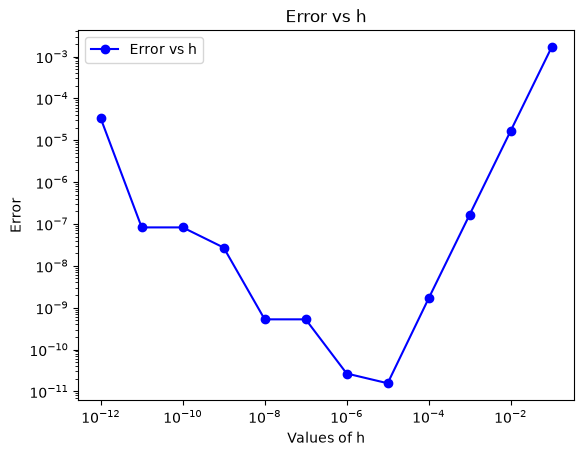
\includegraphics[width=0.8\textwidth]{errorvs_h.png}
    \caption{Error vs h}
\end{figure}

When I graphed the error values vs the h values, the figure showed decreasing values of error as the $h$ values became smaller.
The error is mitigated until $h = 10^{-5}$, where minimum error is reached. As $h$ continues to decrease, the error increases exponentially,
appearing to approach infinity as $h$ goes to zero.

\section{Taylor-Series Error Arguments}

As the value of $h$ decreases, the accuracy of the numerical differentiation increases. This is due to truncation error,
as $h$ is too big in size to give a close result at the point $x = 0$. In our case, the maximum precision is obtained at $h=10^{-5}$. 
As the values continue to get smaller, however, the error increases exponentially due to rounding error. As the values of $h$ approach $0$, 
the centered difference formula requires the subtraction of near-equal values, which is detrimental to computing accuracy and causes a loss 
of significant digits. Furthermore, the error is then compounded by the division of a very small number. \par
Taylor's expansion arguments prove that the truncation error is equal to: 
$$ E_{\mathrm{trunc}} = \left| \frac{h^{2}}{6} f'''(\xi) \right| = C_{1} h^{2} $$
What this demonstrates is that the error is proportional to the square of the $h$-value (Sauer, Timothy \textit{Numerical Analysis})
If $h$ goes from 1 to 10, the error increases by a factor of 100. 

\section{Comparison of Forward, Backward, and Centered Differences}

In this discussion, we have thus far been using the centered difference method. This method differentiates by using values from both the 
right and the left of the point in consideration. It is worth the effort to compare this to forward and backward centered difference methods,
to see which is most effective and has the least error. We will be using the forward difference formula:
$$ f'(x) = \frac{f(x+h) - f(x)}{h} $$
And the backward difference formula:
$$ f'(x) = \frac{f(x) - f(x-h)}{h} $$
The function $f(x)$ will be the same as above, $ f(x) = \sin(x) - \cos(x) $. The following table shows the respective values of the 
difference functions evaluated at $x=0$ with $h$ values from $10^{-1}$ to $10^{-12}$.

\begin{table}
\centering
\begin{tabular}{|c|l|l|l|}
\hline
$h$ & Forward & Centered & Backward \\
\hline
1.0e-01 & 1.048292513688 & 0.998334146468 & 0.948375819249 \\
1.0e-02 & 1.004983291750 & 0.999983333417 & 0.994983375083 \\
1.0e-03 & 1.000499833292 & 0.999999833333 & 0.999499833375 \\
1.0e-04 & 1.000049998333 & 0.999999998333 & 0.999949998333 \\
1.0e-05 & 1.000004999985 & 0.999999999984 & 0.999994999984 \\
1.0e-06 & 1.000000500073 & 0.999999999973 & 0.999999499873 \\
1.0e-07 & 1.000000049434 & 0.999999999474 & 0.999999949514 \\
1.0e-08 & 1.000000005025 & 0.999999999474 & 0.999999993923 \\
1.0e-09 & 0.999999971718 & 1.000000027229 & 1.000000082740 \\
1.0e-10 & 1.000000082740 & 1.000000082740 & 1.000000082740 \\
1.0e-11 & 1.000000082740 & 1.000000082740 & 1.000000082740 \\
1.0e-12 & 0.999977878280 & 1.000033389431 & 1.000088900582 \\
\hline
\end{tabular}
\caption{Returned values with Forward, Backward, and Centered Difference Formulas}
\end{table}

The results in this tabel are what we might expect, given the approach of the respective difference formulas. Up until $h=10^{-9}$, Forward 
$>$ Centered $>$ Backward. This visibly illustrates how the forward difference formula approaches $x=0$ from the higher values, and the 
backward difference formula approaches $x=0$ from the lower values. After this point, however, rounding error and loss of significance begin to have 
visible, catastrophic effect, culminating in the final evaluation at $h=10^{-12}$, where Backward $>$ Centered $>$ Forward. It can be assumed 
that error was accumulating earlier, and only became obvious from $h=10^{-9}$ on. Ultimately, we can see that the Centered Difference Formula is the least 
susceptible to error, as it is consistently between the other two formulas. This is further shown by a table comparing the error values.

\begin{table}[ht]
\centering
\begin{tabular}{|c|c|c|c|}
\hline
$h$ & Forward Error & Backward Error & Centered Error \\
\hline
1.0e-01 & 4.82925e-02   & 1.66583e-03    & 5.16242e-02    \\
1.0e-02 & 4.98329e-03   & 1.66666e-05    & 5.01662e-03    \\
1.0e-03 & 4.99833e-04   & 1.66667e-07    & 5.00167e-04    \\
1.0e-04 & 4.99983e-05   & 1.66711e-09    & 5.00017e-05    \\
1.0e-05 & 4.99998e-06   & 1.56534e-11    & 5.00002e-06    \\
1.0e-06 & 5.00073e-07   & 2.67555e-11    & 5.00127e-07    \\
1.0e-07 & 4.94337e-08   & 5.26356e-10    & 5.04864e-08    \\
1.0e-08 & 5.02476e-09   & 5.26356e-10    & 6.07747e-09    \\
1.0e-09 & 2.82819e-08   & 2.72292e-08    & 8.27404e-08    \\
1.0e-10 & 8.27404e-08   & 8.27404e-08    & 8.27404e-08    \\
1.0e-11 & 8.27404e-08   & 8.27404e-08    & 8.27404e-08    \\
1.0e-12 & 2.21217e-05   & 3.33894e-05    & 8.89006e-05    \\
\hline
\end{tabular}
\caption{Comparison of Finite Difference Method Absolute Errors.}
\end{table}

\clearpage

\section{Conclusion}

In this paper we discussed the Centered Difference Formula for approximating derivatives at a point. We observed how decreasing $h$ value mitigates 
truncation errors, but reducing $h$ past a certain point results in magnified rounding error. The computation of the Centered Difference Formula was 
demonstrated. We considered the Taylor-series arguments for error and the supremacy of Centered Differences over Forward and Backward Differences.

\section{Bibliography}

Sauer, Timothy (2017). \textit{Numerical Analysis}. 3rd ed. Pearson. 
ISBN: 9780134696454

\end{document}